\documentclass{article}
\usepackage{listings}
\lstset{
    basicstyle=\small\ttfamily, % Set font style and size
    breaklines=true,           % Enable line breaking
    % Add more customization options here
  }
  
\usepackage[a4paper,
            bindingoffset=0.2in,
            left=1in,
            right=1in,
            top=1in,
            bottom=1in,
            footskip=.25in]{geometry}

\usepackage{float}
\usepackage{amsmath,amssymb,amsfonts}
\usepackage{hyperref}
\usepackage{graphicx}
\usepackage{tikz}
\usepackage{tikzit}
\input{circuits.tikzstyles}

\definecolor{normGreen}{RGB}{214, 243, 221}
\definecolor{normRed}{RGB}{249, 196, 196}

\title{How to use Cir2Tikz}
\author{Xiaoning Bian \\Tsinghua University}

\begin{document}
\maketitle


\section{Introduction}

Cir2Tikz is tool for converting a circuit encoding to a tikz file for
use in Latex and visual editing in TikZiT.


\begin{figure}[!htb]

  \centering \scalebox{0.8}{\tikzfig{tc2}} 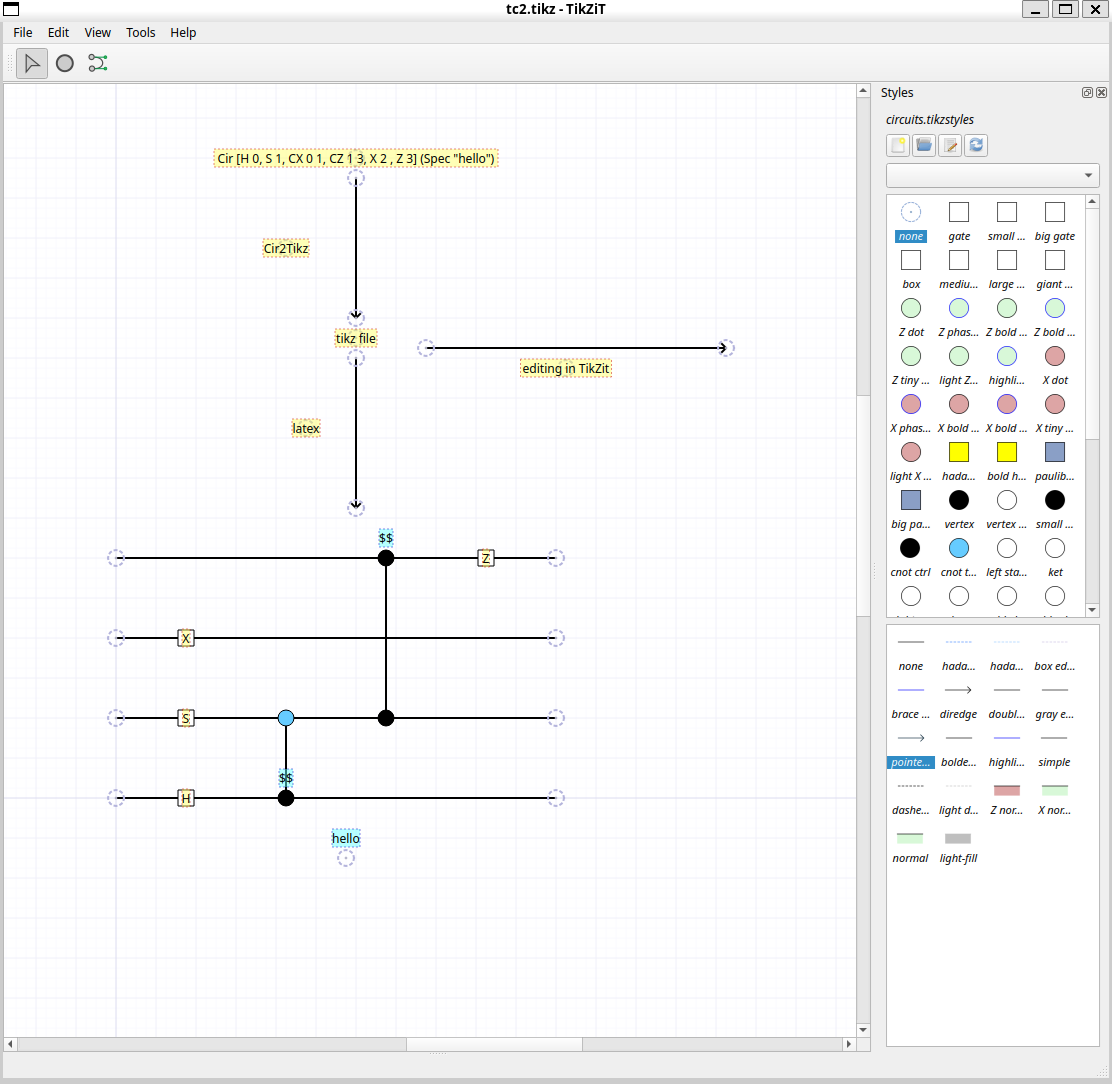
\includegraphics[width=0.35\textwidth]{tikzit}

  \caption{Left part of this figure is drawn in TikZiT whose GUI is
    the right part}
\end{figure}

\section{Steps of using Cir2Tikz}
\begin{itemize}
\item[1.] Open the app here: \url{https://onlinegdb.com/ZV-cO_wwF}
\item[2.] Modify ``your\_cir'' (around line 12) in the app as you
  like.
\item[3.] Click ``Run'' button on the top left corner of the app. Try
  again if it outputs nothing.
\item[4.] Select the output starting with ``$\setminus$begin'' line ending with
  ``$\setminus$end'' line; Copy it; Paste it to an empty .tikz file; Save.
\end{itemize}

\section{Compiling with latex}
This is the minimal tex file setup:
\lstinputlisting{test.tex}

That means you need download the file ``circuits.tikzstyles'' and save
it in the same folder as your .tex file. Here is the file:

\hspace{2cm} \url{https://www.dropbox.com/scl/fi/5ubc4uo7g4z6yv7cmyp9p/circuits.tikzstyles?rlkey=abndq6652j3t1gawzpbg2c1ud&st=lezzil4l&dl=0}

Similarly, download and save the file ``tikzit.sty'' here:

\hspace{2cm} \url{https://www.dropbox.com/scl/fi/riqyuvj1sbn48osxbnlk9/tikzit.sty?rlkey=y4zhykbgq3y5adkk0q6llqx3e&st=5bztui95&dl=0}

\vspace{0.5cm}

Note that sometime you might need to install missing packages such as
\verb|xcolor|.

\section{Editing in TikZiT}
\begin{itemize}
\item[1.] Install TikZiT from here: \url{https://tikzit.github.io/}
\item[2.] Load the style file ``circuits.tikzstyles'' you just
  downloaded by clicking this button:
  \begin{figure}[h]
    \centering 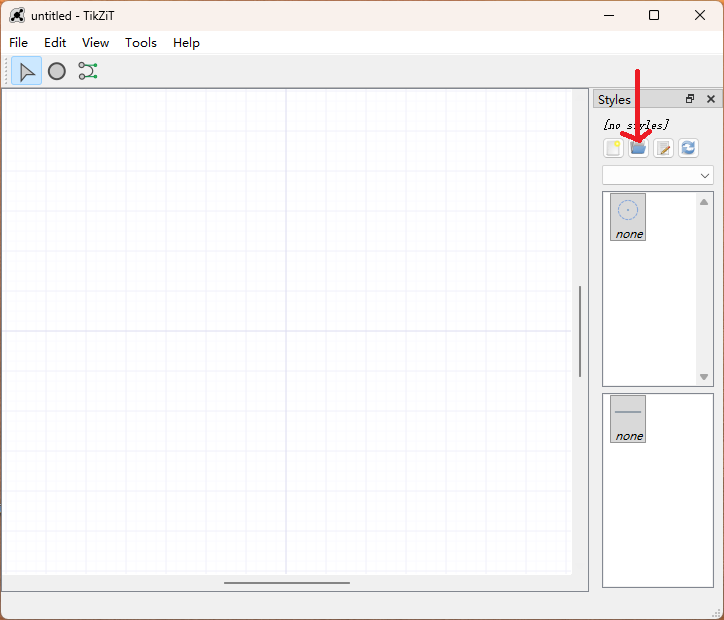
\includegraphics[width=0.5\textwidth]{load-style}
  \end{figure}

\item[3.] Click ``File $\rightarrow$ Open'' to open your tikz file and
  then edit it.
\item[4.] Click ``Tools $\rightarrow$ Make Preview'' to preview your
  circuit. (For this to work, you need latex installed in your system
  so that TikZiT can call it; see
  \href{https://tikzit.github.io/#preview}{Previewing} for help) A preview would look like:
  \begin{figure}[H]
    \centering 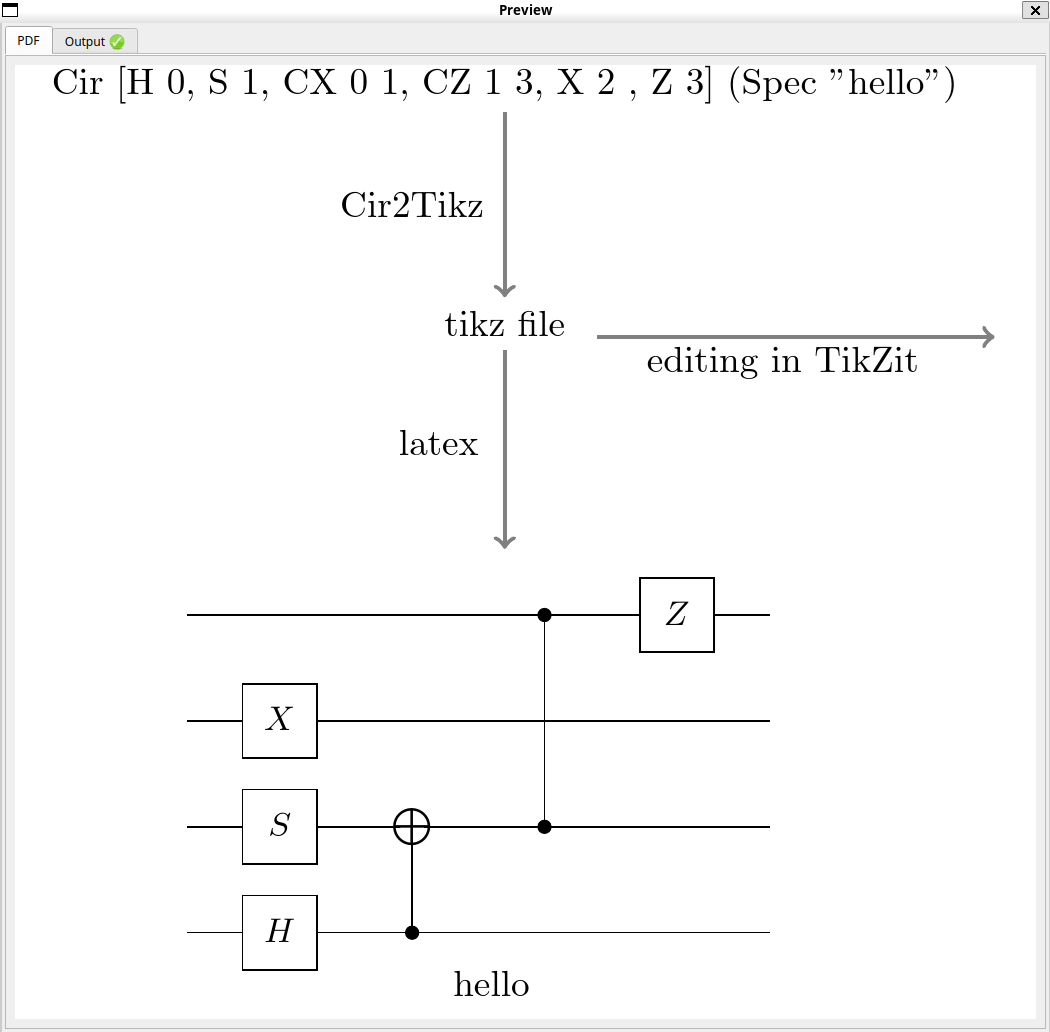
\includegraphics[width=0.5\textwidth]{preview}
  \end{figure}
  
  
\end{itemize}

\section{Advanced use}\label{sec:au}

\subsection{Draw a list of circuit equations (with specifications)}
For example, the encoding of a list of equations in Fig \ref{fig:es}:
will be compiled to Fig \ref{fig:des}.

\begin{figure}[h] \centering
  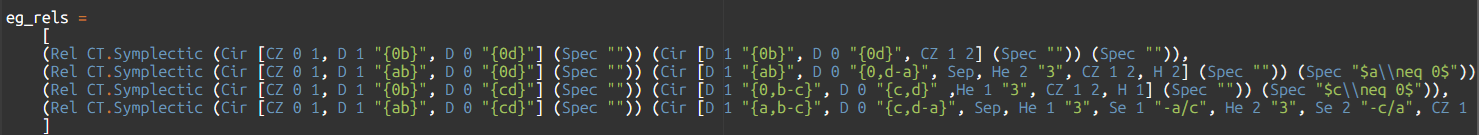
\includegraphics[width=1\textwidth]{eg-rels}
  \caption{Encoding of a list of circuit equations}
  \label{fig:es} 
\end{figure}
  
  
\begin{figure}[h]
  \centering \scalebox{0.7}{\tikzfig{test_cir}}
  \caption{Draw a list of circuit equations}
  \label{fig:des}
\end{figure}

\subsection{Draw a list of positioned circuits }

For example, the encoding of a list of positioned circuits in Fig
\ref{fig:epc} will be compiled to Fig \ref{fig:pc}.

\begin{figure}[H]
\begin{verbatim}
eg_pcirs :: [(Cir , PositionSpec)]
eg_pcirs =
  [
    (Cir eg1 (Spec "eg1") , PositionSpec Up "\\Rightarrow"),
    (Cir eg2 (Spec "eg2") , PositionSpec Right "\\mapsto"),
    (Cir eg1 (Spec "eg1 again") , PositionSpec RU "\\rightarrow"),
    (Cir eg2 (Spec "eg2 again") , PositionSpec RU "\\rightarrow")
  ]
\end{verbatim}
  \caption{Encoding of a list of positioned circuits}
  \label{fig:epc}
\end{figure}


Note that the supported ``directions'' are
\verb|Up , Down , Right , Left , LU , LD , RU , RD|.  Also note that
in \verb|[(cir1, pspec1), (cir2, pspec2) ... ]|, \verb|pspec1|
specifies the relative position of \verb|cir2| w.r.t \verb|cir1|, and
the connective between them. The last pspec is discarded.

  
\begin{figure}[h]
  \centering \scalebox{0.6}{\tikzfig{tc3}}
  \caption{Draw a list of positioned circuits}
  \label{fig:pc}
\end{figure}

\section{Pros and Cons}
\subsection{Pros}
\begin{itemize}
\item[1.] Lightweight: the number of loc is less than 1000.
\item[2.] Qiskit's
  \verb| latex_code = qc.draw(output='latex_source') | outputs
  \verb| qcircuit | format .tex code which lacks TikZiT visual editing
  tool.
\item[3.] \verb|qcircuit| format .tex code also lacks support for
  drawing multiple circuit in one figure. So it cannot support
  advanced use as in Section \ref{sec:au}.
\item[4.] Extensible: we welcome customization requests to suit your
  specific needs.
\end{itemize}


\subsection{Cons}
\begin{itemize}
\item[1.] Limited functionality: for the moment, it does not support
  measurement, initialization, termination etc. It only supports
  unitary circuit.
\item[2.] Coded in Haskell which is less used.
\item[3.] This is the first release. So it might be buggy.
\end{itemize}



\end{document}

